%- Da die verschiedenen Eigenschaften immer nur kurz erklärt werden, wird der Zuhörer dazu neigen sie im Lauf des Vortrags zu verwechseln oder die genaue Bedeutung nicht mehr aus der Erinnerung heraus abrufen können. Wiederhole daher (mündlich) die Bedeutung der Eigenschaften kurz wenn du sie verwendest. Dieser Vorschlag ist vor allem für die Zeitpunkte im Vortrag gedacht, wenn du schon mehrere Eigenschaften eingeführt hast. Man könnte alternativ irgendwo in eine Ecke der Folie die Bedeutungen der Eigenschaften wiederholen, die gerade benötigt werden. Das stelle ich mir aber als eine etwas schwierigere Aufgabe vor, da auch darauf geachtet werden muss, dass die Folien nicht zu voll wirken.

\documentclass{sikslides}

\usepackage{bm}
\usepackage{tabu}
\tabulinesep=1.2mm
\usepackage{subcaption}
\usepackage{graphicx}

\newcommand*{\vcenterimage}[2]{\vcenter{\hbox{\includegraphics[height=#1]{#2}}}}
\newcommand*{\vcenterarrow}{\vcenter{\hbox{$\bm{\Longrightarrow}$}}}

\title[Security Considerations for CPS]{Security Considerations for Cyber-Physical Systems}
\subtitle{Seminar \\Cyber-Physical Systems} % Bachelor
\author{Maximilian Ammann}
\date[01.02.2019]{01. Februar 2019}
\setbeamercovered{invisible}
\setbeamertemplate{section in toc}[sections numbered]
\setbeamertemplate{subsection in toc}[subsections numbered]
\begin{document}

    \titleframe

    \section{Motivation}
    \begin{frame}[noframenumbering,plain]
        \frametitle{Starker Anstieg an Sicherheitslücken}
        \centering
        \begin{center}
            \includegraphics[trim=0 25px 0 25px,height=7.3cm]{figure/nvd_stats.png}
            \textbf{Was bedeutet das für Cyber-physical Systems?}
        \end{center}
        \hfill \tiny Quelle:\thinspace{\tiny\itshape NVD 25.01.2019}
    \end{frame}

    \begin{frame}
        \frametitle{Gliederung}
        \tableofcontents[pausesections]
        %\tableofcontents[pausesections]
        %\tableofcontents
    \end{frame}

    %    \sectionframe{Eigenschaften von CPS und Angriffsszenarios}
    \section{Eigenschaften von CPS und Angriffsszenarios}

    \begin{frame}[label=abstrakt]
        \frametitle{Abstraktion eines Cyber-physical Systems}
        \begin{figure}
            \centering
            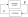
\includegraphics[width=5cm]{../figure/abstrakt}
        \end{figure}

        \begin{itemize}
            \item Bidirektionale Kommunikation zwischen Cybersystem und physischen System
            \item $y$ und $u$ und die Systeme selbst stellen mögliche Angriffspunkte dar
        \end{itemize}

        \pause

        \vspace{10px}
        $\rightarrow$ Erweiterte Angriffsfläche im Vergleich zu Cybersystemen
    \end{frame}

    \begin{frame}
        \frametitle{Sicherheitseigenschaften von CPS}
        \centering
        $\vcenterimage{2.5cm}{../figure/cia}\vcenterarrow\vcenterimage{3.5cm}{../figure/triad}$
        \vspace{10px}
        \begin{itemize}[<+->]
            \item Wichtige Eigenschaften bei der Entwicklung von Systemen
            \item CIA-Dreieck ist in Literatur zu Cybersicherheit weit verbreitet
            \item Erweiterungen des CIA-Dreiecks sind nicht einheitlich in der Literatur (CIAANV-Hexagon?!)
            \pause
        \end{itemize}
        \vspace{10px}

        $\rightarrow$ Komplexere Situation durch komplexere Sicherheitsanforderungen an CPS
    \end{frame}

    \begin{frame}
        <1>[label=eigenschaften]
        \frametitle{Eigenschaften}

        \begin{overlayarea}{\textwidth}{10cm}
            \begin{tabu}
                to \linewidth { | X[1.6,l] | X[5,l] | }
                \hline
                Eigenschaft: $e$&Ein System hat Eigenschaft $e$ genau dann, wenn~\ldots \\
                \hline
                \only<1>{\bf}
                Availability&
                \only<1>{\bf}
                \ldots Ressourcen für autorisierte Teilnehmer angemessen verfügbar ist. \\
                \hline
                \only<2>{\bf}
                \uncover<2->{Confidentiality}&
                \only<2>{\bf}
                \uncover<2->{\ldots nur autorisierte Teilnehmer auf Ressourcen zugreifen können.}\\
                \hline
                \only<3>{\bf}
                \uncover<3->{Integrity}&
                \only<3>{\bf}
                \uncover<3->{\ldots Ressourcen nur von autorisierten Teilnehmern verändert werden können.} \\
                \hline
                \only<4>{\bf}
                \uncover<4->{Authenticity}&
                \only<4>{\bf}
                \uncover<4->{\ldots sich beide Kommunikationspartner einig über die Identität des Gegenübers sind.} \\
                \hline
                \only<5>{\bf}
                \uncover<5>{Veracity und Plausibility} &
                \only<5>{\bf}
                \uncover<5>{\ldots Aussagen des Systems der Wahrhaftigkeit der Wirklichkeit entsprechen.} \\
                \hline
                %Non-repudiation &
                %\ldots jedes Ereignis, welches das System beeinflusst, nachvollzogen werden kann. \\
                %\hline
            \end{tabu}
        \end{overlayarea}
    \end{frame}

    \subsection{Denial-of-Service Angriff}
    \begin{frame}
        \frametitle{Szenario: Denial-of-Service Angriff}
        \begin{figure}
            \centering
            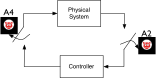
\includegraphics[width=4cm]{figure/dos}
            % \caption{Abstraktion eines DoS Angriffs}
        \end{figure}
        \begin{itemize}
            \item Ziel: Mit großer Flut an Informationen die \textbf{Availability} des CPS stören
            \pause
            \item Beispiele:
            \begin{itemize}
                \item CAN Busse in Autos: Fehlfunktion der Warnlichter, Diebstahlsicherung
                \item Echtzeitkritische Stromnetze: Störung des Normalbetrieb
            \end{itemize}
            \pause
            \item Bei mehreren Angreifern: Distributed-DoS
            \item Kabellose Kommunikation meist anfälliger wegen geringer Bandbreite
        \end{itemize}
    \end{frame}

    \subsection{Man-in-the-Middle Angriff}
    % Continue to Confidentiality, Integrity, Authenticity
    \againframe<2>{eigenschaften}
    \againframe<3>{eigenschaften}
    \againframe<4>{eigenschaften}

    \begin{frame}[t]
        \frametitle{Szenario: Man-in-the-Middle Angriff}
        \begin{overlayarea}{\linewidth}{4cm}
            \begin{figure}
                \centering
                \includegraphics[width=4cm]{figure/mitm}
                % \caption{Abstraktion eines MITM Angriffs}
            \end{figure}
        \end{overlayarea}
        \begin{onlyenv}<1-2>
        \begin{itemize}
            \item Passiv: Nur lauschen
            \begin{itemize}
                \item Verletzung der \textbf{Confidentiality} des CPS
                \pause
            \end{itemize}
            \item Aktiv: Verändern der Daten
            \begin{itemize}
                \item Bei fehlender \textbf{Authenticity}: Keine Verifikation der Identität möglich
                \item Bei fehlender \textbf{Integrity}: Keine überprüfung auf Veränderung der Daten (Prüfsummen!)
            \end{itemize}
            \pause
        \end{itemize}
        \end{onlyenv}

        \begin{onlyenv}<3-4>
        \begin{itemize}
            \item Beispiele:
            \begin{itemize}
                \item ARP-Poisoning in IEE 802.11 und Local Area Networks
                \pause
                \item Offline Replay Angriffe bei Autos
            \end{itemize}
        \end{itemize}
        \end{onlyenv}

    \end{frame}

    \subsection{Angriff auf das physische System}
    % Continue to Veracity
    \againframe<5>{eigenschaften}
    \begin{frame}
        \frametitle{Szenario: Angriff auf das physische System}
        \begin{figure}
            \centering
            \includegraphics[width=4cm]{figure/physical}
            % \caption{Abstraktion eines physischen Angriffs}
        \end{figure}
        \begin{itemize}
            \item Ziel: Verändern der Daten bevor diese an das Cybersystem geschickt werden
            \item Authenticity hilft nicht \textbf{Veracity} sicherzustellen
            \pause
            \item Beispiele:
            \begin{itemize}
                \item Manipulation von physischen Prozessen führt zu Wechselwirkungen
                \item Manipulation von Sensoren
            \end{itemize}
        \end{itemize}
    \end{frame}

    % Continue to Non-repudiation
    % \againframe<6>{eigenschaften}

    %    \bgroup
    %    \setbeamercolor{background canvas}{bg=black}
    %    \begin{frame}[plain]{}
    %        \centering
    %        \Huge\textbf{\textcolor{white}{Time to zoom out!}}
    %    \end{frame}
    %    \egroup

    \section{Gegenmaßnahmen}
    \sectionframe{Gegenmaßnahmen}
    \subsection{Proaktive Maßnahmen: Verhindern von Angriffen}
    \sectionframe{Proaktive Maßnahmen: Verhindern von Angriffen}
    \begin{frame}[t]
        \frametitle{Proaktive Maßnahmen: Verhindern von Angriffen}
        \frametitle{Proaktive Maßnahmen: Verhindern von Angriffen}
        \begin{overlayarea}{\linewidth}{1cm}
            \begin{block}{}
                Proaktive Maßnahmen: Maßnahmen, die vor dem Angriff getroffen werden müssen
            \end{block}
        \end{overlayarea}

        \vspace{2cm}
        \begin{itemize}[<+->]
            \item Authentisierung der Kommunikationspartner durch z.B. Signaturen $\rightarrow$ \textbf{Authenticity}
            \item Verschlüsselung der Kommunikationsdaten $\rightarrow$ \textbf{Confidentiality}
            \item Prüfsummen zur Validierung der Kommunikation $\rightarrow$ \textbf{Integrity}
        \end{itemize}
    \end{frame}
    \begin{frame}
        \frametitle{Proaktive Maßnahmen: Verhindern von Angriffen}
        \begin{itemize}[<+->]
            \item Transportverschlüsselung: TLS für TCP, DTLS für UDP, Logicial Link Transport Protocol für NFC $\rightarrow$ \textbf{Confidentiality, Integrity, Authenticity}
            \item Redundanzen und Diversität für CPS $\rightarrow$ \textbf{Availability}
            \item Hardware Security Module: Verhindern Auslesen von Secrets wie Schlüssel
            \item Verifikation von Programmen: Reduzieren von Lücken durch z.B.\ Code-Audits oder Fuzzing
        \end{itemize}
    \end{frame}
    \begin{frame}
        \frametitle{Proaktive Maßnahmen: Verhindern von Angriffen}
        \begin{itemize}
            \item Trennung von Netzwerken
            \item Trennung von Privilegien
            \item Least Privilege-Prinzip
        \end{itemize}
    \end{frame}
    \begin{frame}
        \frametitle{Proaktive Maßnahmen: Verhindern von Angriffen}
        \begin{itemize}[<+->]
            \item Gesetzgebung als Abschreckung einen Angriff durchzuführen
            \item Physische Baumaßnahmen zum Schutz vor Manipulation\\(Allerdings ist ein Cyberangriff sehr viel Wahrscheinlicher)
        \end{itemize}
    \end{frame}

    \subsection{Reaktive Maßnahmen: Detektion und Wiederherstellung}
    \sectionframe{Reaktive Maßnahmen: Detektion und Wiederherstellung}
    \begin{frame}
        \frametitle{Reaktive Maßnahmen: Detektion und Wiederherstellung}
        \begin{block}{}
            Reaktive Maßnahmen: Maßnahmen, die auf Angriffe reagieren
        \end{block}
        \begin{itemize}
            \item Beispiele:
            \begin{itemize}
                \item Überwachung von Sensoren eines Kraftwerkes $\rightarrow$ \textbf{Veracity}
                \item Wiederherstellung der physischen und Cybersystemen mithilfe von Checkpoints $\rightarrow$ \textbf{Veracity}
            \end{itemize}
        \end{itemize}
    \end{frame}

    \begin{frame}
        \frametitle{Anomaliedetektion in einem Kraftwerk}
        \begin{figure}
            \centering
            \begin{subfigure}{0.49\textwidth}
                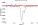
\includegraphics[height=3cm]{../figure/entropy_a}
                \caption{Gefälschte Werte eines Sensors}
                \label{entropy_a}
            \end{subfigure}
            \begin{subfigure}{0.49\textwidth}
                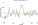
\includegraphics[height=3cm]{../figure/entropy_b}
                \caption{Entropie des gesamten Kraftwerks}
                \label{entropy_b}
            \end{subfigure}
        \end{figure}

        \begin{itemize}[<+->]
            \item In (a) werden einem Sensor gefälschte Werte vorgespielt
            \item In (b) ist die Fälschung durch einen Verschobenen Mittelwert der Entropie zu erkennen
            \item Es ist nicht in jedem Fall möglich den verantwortlichen Sensor zu bestimmen
        \end{itemize}
    \end{frame}

    \section{Zusammenfassung und Fazit}
    \begin{frame}
        \frametitle{Zusammenfassung}
        \begin{itemize}
            \item<1-> Erweiterte Angriffsfläche im Vergleich zu Cybersystemen
            \item<2-> Erweiterung des CIA-Dreieck zu einem Hexagon
            \begin{itemize}
                \item Availability
                \item Confidentiality
                \item Integrity
                \item Authenticity
                \item Veracity
            \end{itemize}
            \\$\rightarrow$ Komplexere Sicherheitsanforderungen an CPS
            \item<3-> Angriffsvektoren sind andere als bei klassischen Cybersystemen
        \end{itemize}
    \end{frame}

    \begin{frame}
        \frametitle{Fazit}

        \begin{center}
            \bf Sicherheit für CPS bedarf spezieller Betrachtung
        \end{center}

        \begin{itemize}[<+->]
            \item Durch anstieg an Sicherheitslücken im Cybersystem sind auch physische Systeme betroffen\\$\rightarrow$ Neue Sicherheitskonzepte nötig falls Cybersystem nicht vertrauenswürdig
            \item Kombination auf Cybersystemen und physischen Systemen stellen neue Herausforderungen dar
%            \item Man muss CPS oft mehr vertrauen entgegenbringen als Cybersystemen
            \item Altsysteme stellen besondere Herausforderung dar (Supervisory Control and Data Acquisition Systeme)
        \end{itemize}
    \end{frame}
\end{document}

